\subsection{Overview}
Increasingly, internet users are utilizing multiple devices to assist with their daily tasks. According to a study by Criteo\footnote{\href{https://www.criteo.com/de/blog/die-chancen-von-cross-device-optimal-nutzen/}{https://www.criteo.com/de/blog/die-chancen-von-cross-device-optimal-nutzen/}}, 31\% of purchases involve the use of multiple devices. Users tend to review a product several times from different devices before making a purchase decision. Consequently, company owners, website and app developers have become interested in cross-device tracking to enhance conversion rates and gain deeper insights into consumer behavior. In our research, we aim to explain what cross-device tracking is, its purpose, the potential risks it poses to website users, and demonstrate its usage through practical examples. Additionally, we will compare two categories of websites to identify signs of cross-device tracking implementation.

\subsubsection{Definition}
Cross-device tracking is the process of monitoring user behavior across various devices, such as PCs, smartphones, and tablets, to create the most comprehensive user profile possible by gathering as much information about the user as possible. There are different types of cross-device tracking, which will be described in more detail in Chapter 1.3.

It should be noted that in the modern world, the scope of cross-device tracking is expanding, for instance, with the use of smart homes, as the number of devices increases over time, allowing this technology to be integrated into all areas of a user's life. Additionally, with the development of artificial intelligence, this technology is becoming increasingly precise in recognizing information about users.

\subsubsection{Purpose}
One of the primary reasons companies are exploring cross-device tracking is to improve their marketing strategies and make their advertising more targeted. By understanding their customers better through a more complete profile, which includes their activities across multiple devices, companies can more accurately predict both immediate and future buying habits. This not only allows for better-customized advertising that resonates with specific user groups but also helps companies save money by not wasting resources on ineffective ads. While this technology is not universally used yet, its adoption is growing among many companies\footnote{\href{https://cdt.org/wp-content/uploads/2015/10/10.16.15-CDT-Cross-Device-Comments.pdf}{https://cdt.org/wp-content/uploads/2015/10/10.16.15-CDT-Cross-Device-Comments.pdf}}.

Adobe's Cross-Device Analytics, a feature of Adobe Analytics, is a great example of using and implementing this technology. It offers a user-centric view, linking a user's activities across multiple devices like smartphones, tablets, and computers. Key features include Field-Based Stitching, which connects user activities on different devices based on deterministic methods, and Device Graph, which analyzes connections between devices. This helps in attributing user actions accurately, such as linking an ad click on one device to a purchase on another, offering valuable insights for marketing strategies while considering user privacy\footnote{\href{https://experienceleague.adobe.com/docs/analytics/components/cda/overview.html?lang=en}{https://experienceleague.adobe.com/docs/analytics/components/cda/overview.html?lang=en}}.

However, sales are not the only area where cross-device tracking can be useful. It's also an excellent resource for political parties or media outlets to find their audience, tailoring the right messages or news to specific target groups. The principle is the same: the more information you have about a user, the easier it is to tailor your approach to them. The more sources of information (i.e., devices), the more you can track the behavior and interests of the user.
\subsection{Importance in Modern Digital Exosystem}

\subsubsection{Evolution of User Behavior}
The digital landscape has seen a major evolution in user behavior, particularly in the way people interact with technology. In the early stages of the internet, user behavior was device-specific, primarily bounded to desktop computers. This era was characterized by more predictable online activities, with users typically accessing the internet from fixed locations and a small amount of different devices, which made user tracking relatively easy.

\vspace{0.8cm}
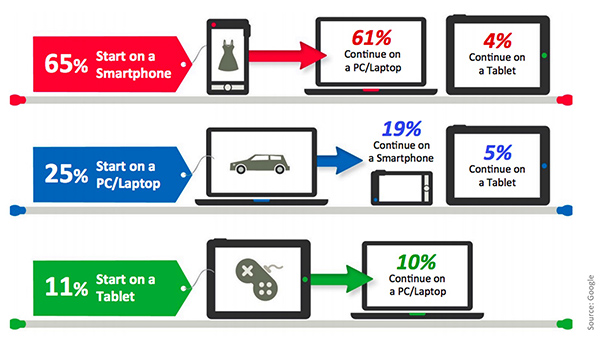
\includegraphics[width=0.95\textwidth]{./assets/google-cdt-stats.jpeg}
\vspace{0.8cm}

The invention of mobile technologies, especially smartphones changed online activities significantly and lead to a transformation in user behavior. Users began interacting with digital content across multiple platforms and often seamlessly switching between devices. For reference, Google published an interesting statistic, that shows more than 80 percent of all users switching their device during the user journey. Multi-platform interaction introduced a new level of complexity in understanding user behavior as users were no longer restricted to a single device.

Moreover, the rise of smart devices and the Internet of Things in the last years are the reason for  even more complex interactions between devices. Today, a wide network of connected devices are creating a diverse and complex digital footprint.

\subsubsection{Challenges in User Tracking}
Parallel to the evolution of users online behavior, the task of tracking users across multiple devices has become increasingly challenging. As there exists no universal login system or consistent identifiers across different websites, establishing a meaningful user profile from disparate device usage is really complex.

Privacy considerations make cross-device tracking even more complicated. With increasing sensitivity to data privacy and the introduction of strong regulations like the General Data Protection Regulation (GDPR) and the California Consumer Privacy Act (CCPA), tracking users across devices must navigate the line between effective data collection and respect for user privacy and consent.

The diversity of devices and platforms results in fragmented data sources, requiring advanced technological solutions for data integration and analysis. The need for algorithms and technologies is necessary to not only gather but also accurately interpret the large amount of data generated by multi-device usage.

Looking ahead, these challenges will even intensify with the continuous evolution of technology. The integration of artificial intelligence and machine learning will potentially lead to advancements in user tracking, but also brings additional complexities regarding privacy regulations. The task of user tracking demands innovative solutions that are adaptable, take privacy into account and are able of decoding increasingly complex device interactions.

\subsection{Techniques Employed in CDT}
\subsubsection{Deterministic Tracking}
\subsubsection{Probabilistic Tracking}
\subsubsection{Browser Fingerprinting}
\subsubsection{Cookies and Tracking Pixels}
\subsubsection{Location Data}